\documentclass[a4paper,12pt]{article}

\usepackage{amsmath,amssymb,multicol,tikz}
\usepackage[margin=2cm]{geometry}
%\usetikzlibrary{calc}
\usepackage{amsmath}
\usepackage{amsthm}
\usepackage{thmtools}
\usepackage{hyperref}
\usepackage{enumerate}
\usepackage{xcolor}
\usepackage{fancyvrb}

\pagestyle{empty}

\newcommand\Q{\mathbf{Q}}
\newcommand\R{\mathbf{R}}
\newcommand\Z{\mathbf{Z}}

\usepackage{array}
\newcolumntype{P}[1]{>{\centering\arraybackslash}p{#1}}

\newcommand\indd{${}$\hspace{20pt}}

\declaretheoremstyle[headfont=\normalfont\bfseries,notefont=\mdseries\bfseries,bodyfont = \normalfont,headpunct={:}]{normalhead}
\declaretheorem[name={Uzdevums}, style=normalhead,numberwithin=section]{problem}

\setcounter{section}{1}

\setlength\parindent{0pt}

\begin{document}

\clearpage
\begin{center}
\parbox{3.5cm}{\flushleft\bf Uzdevumu lapa \newline ATV} \hfill {\bf\LARGE Dažādas tēmas} \hfill \parbox{3.5cm}{\flushright\bf 2022-01-(18|20)} %\\[2pt]
\end{center}

%\hrule\vspace{2pt}\hrule
\hrule

\vspace{20pt}
{\Large \bf Varbūtību atkārtojums}


\vspace{10pt}
\begin{problem}
(Par bērnu dzimumiem.) Pieņemsim, ka zēni un meitenes piedzimst ar vienādām varbūtībām $p=0.5$. 
Šajos piemēros mūs interesēs tās ģimenes, kurās ir tieši divi bērni (bez papildus viltībām: 
pieņemam, ka abi bērni ir atšķirami, nav dvīņi un dzīvo kopā ar abiem vecākiem).
Noskaidrosim, ar kādām varbūtībām tajās sastopami bērnu dzimumi. 
\begin{enumerate}
\item Pirmajā eksperimentā no lielas valsts iedzīvotāju reģistra atlasīja ģimenes ar
tieši diviem bērniem, turklāt no tām izvēlējās tikai tās, kurās ir vismaz viens zēns.
Ar kādu varbūtību, nejauši izvēloties ģimeni no šādi atfiltrēta saraksta, abi bērni būs zēni?
\item Otrajā eksperimentā pētnieki devās uz masu pasākumu, kurā epidemioloģisko 
ierobežojumu dēļ ielaiž tikai vienu no bērniem.
Pieņemsim, ka līdzi ņemamo bērnu vecāki izvēlas nejauši ar vienādām varbūtībām.
Kādā sastaptajā ģimenē bija līdzi paņemts zēns -- un sastaptie cilvēki apstiprināja, 
ka viņu ģimenē ir tieši vēl viens bērns, kurš palicis mājās.
Ar kādu varbūtību šajā ģimenē abi ir zēni? 
\end{enumerate}
\end{problem}


\vspace{10pt}
\begin{problem}
(Par nejaušo klaiņošanu.) 
Iedomāsimies, ka pilsētā ielas veido kvadrātveida režģi: 
$5$ ielas ziemeļu-dienvidu virzienā, 
$5$ ielas rietumu-austrumu virzienā, ar $4 \times 4$ kvartāliem starp tām: 
Sk.\ zīmējumu pa kreisi.

\center{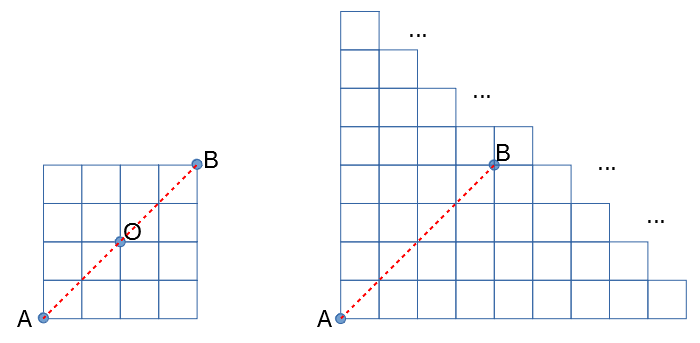
\includegraphics[width=4in]{atv-worksheet-2022-01-18/city-map.png}}

\begin{enumerate}
\item Ceļotājs vēlas no punkta $A$ nonākt punktā $B$; turklāt doties 
pa kādu no īsākajiem ceļiem, ejot tikai uz ziemeļiem vai austrumiem. 
Nonākot kādā no krustojumiem, kurā ir izvēle -- doties uz ziemeļiem vai austrumiem, 
ceļotājs met monētu un izvēlas virzienu ar vienādām varbūtībām $0.5$. 
(Iziet ārpus pilsētas ārējā kvadrāta nedrīkst.)
Noskaidrot ar kādu varbūtību ceļotājs nonāks pašā pilsētas centrā, krustojumā $O$. 
\item Ceļotājs nejauši pārvietojas pa $4 \times 4$ pilsētu -- tāpat kā iepriekšējā 
piemērā. 
Atrast, ar kādu varbūtību viņš nekad nenonāks zem (uz dienvidiem) no nogriežņa $AB$. 
\item Cits ceļotājs pārvietojas pa lielāku pilsētu ar kvadrātveida kvartāliem, 
kura izveidota kā bezgalīgs
kvadrants, kurš neierobežoti plešas uz ziemeļiem un uz austrumiem. 
Ceļojums sākas kvadranta kreisajā apakšējā 
virsotnē -- punktā $A$. Katrā krustojumā viņš met 
monētu un izvēlas virzienu (uz ziemeļiem vai uz austrumiem) ar vienādām varbūtībām $0.5$. 
Noskaidrot ar kādu varbūtību viņš pirmajos $8$ sava ceļa posmos nenonāks zem (uz dienvidiem) no nogriežņa
$AB$, ja zināms, ka viņš nonāca krustojumā $B$. 
\end{enumerate}
\end{problem}



\vspace{20pt}
{\Large \bf Kombinatorikas atkārtojums}




\vspace{10pt}
\begin{problem}
(Par bitu virknēm.)
Dots naturāls skaitlis $n$ ($n \geq 4$). 
Cik ir tādu virkņu garumā $n$, kas 
satur tikai ciparus "$\mathtt{0}$" un "$\mathtt{1}$"; 
turklāt fragments "$\mathtt{01}$" sastopams tieši divās vietās?
\end{problem}


\vspace{10pt}
\begin{problem} 
(Par konfekšu virknēm.)
Aģents $X$ $30$ dienu laikā apēda $45$ konfektes -- 
katru dienu vismaz vienu konfekti. 
Pierādīt, ka var atrast dažas pēc kārtas sekojošas dienas, kurās
$X$ apēda tieši $14$ konfektes.
\end{problem}





\vspace{20pt}
{\Large \bf Ģeometrijas atkārtojums}

\vspace{10pt}
\begin{problem}
Trijstūrī $ABC$ novilkti augstumi $AA_1$ un
$BB_1$; malas $AB$ viduspunkts ir $M$. 
Pierādīt, ka $MA_1 = MB_1$. 
\end{problem}

\vspace{10pt}
\begin{problem}
Izliektā četrstūrī $ABCD$ leņķi $A$ un $C$ ir taisni. 
Pierādīt, ka 
\[ AC = BD \cdot \sin ( \sphericalangle ABC). \]
\end{problem}


\vspace{10pt}
\begin{problem}
Riņķa līnijā ievilkta sešstūra diagonāles $AD$, 
$BE$ un $CF$ krustojas vienā punktā. pierādīt, ka 
$AB \cdot CD \cdot EF = BC \cdot DE \cdot AF$. 
\end{problem}

\vspace{10pt}
\begin{problem}
Riņķa līnijas ar centriem $O_1$ un $O_2$ krustojas
punktos $A$ un $B$. Taisne $O_1A$ krusto 
riņķa līniju ar centru $O_2$ punktā $N$. 
Pierādīt, ka punkti $O_1$, $O_2$, $B$ un $N$ atrodas uz
vienas riņķa līnijas. 
\end{problem}

\vspace{10pt}
\begin{problem}
Riņķa līniju $S_1$ un $S_2$ centri ir attiecīgi $O_1$ un $O_2$. 
Tās krustojas punktos $A$ un $B$. 
Taisne $MN$ pieskaras riņķa līnijai $S_1$ punktā $M$
un riņķa līnijai $S_2$ punktā $N$. 
Ar $A$ apzīmēts tas riņķa līniju krustošanās punkts, 
kas atrodas tālāk no taisnes $MN$. 
Pierādīt, ka 
$\sphericalangle O_1 A O_2 = 2 \sphericalangle MAN$. 
\end{problem}


\vspace{10pt}
\begin{problem}
Dots četrstūris $ABCD$, kas ievilkts riņķa līnijā, turklāt 
$AB = BC$. Pierādīt, ka ${\displaystyle S_{ABCD} = \frac{1}{2}(DA + CD) \cdot h_b}$, 
kur $h_b$ ir augstums trijstūrī $ABD$, kas novilkts no virsotnes $B$. 
\end{problem}

\vspace{10pt}
\begin{problem}
Četrstūris $ABCD$ ievilkts riņķa līnijā, turklāt 
$AC$ ir leņķa $DAB$ bisektrise. 
Pierādīt, ka $AC \cdot BD = AD \cdot DC + AB \cdot BC$. 
\end{problem}


\vspace{10pt}
\begin{problem}
Taisnleņķa trijstūrī $ABC$ no taisnā leņķa virsotnes $C$
novilktas bisektrise $CM$ un augstums $CH$. 
$HD$ un $HE$ ir attiecīgi trijstūru $AHC$ un $CHB$ 
bisektrises. 
Pierādīt, ka punkti $C, D, H, E, M$ atrodas
uz vienas riņķa līnijas. 
\end{problem}

%\vspace{10pt}
%\begin{problem}
%Divas riņķa līnijas iet caur leņķa virsotni un 
%to pašu punktu uz šī leņķa bisektrises. 
%Pierādīt, ka nogriežņi, kurus tās atšķeļ uz 
%leņķa malām, ir vienādi. 
%\end{problem}

\vspace{10pt}
\begin{problem}
Trijstūris $BHC$, kur $H$ ir trijstūra $ABC$ augstumu centrs, 
tiek papildināts līdz paralelogramam $BHCD$. 
Pierādīt, ka $\sphericalangle BAD = \sphericalangle CAH$. 
\end{problem}

\vspace{10pt}
\begin{problem}
Pierādīt, ka tad, ja četrstūris ar perpendikulārām 
diagonālēm ir gan ievilkts (kāda riņķa līnijā), 
gan arī apvilkts (ap kādu citu riņķa līniju), 
tad tas ir simetrisks attiecībā pret vienu no 
savām diagonālēm. 
\end{problem}



\end{document}

